\chapter{Marco Teórico}
\newpage
\section{Power TAC(Trading Agent Competition).}
Es una competencia de simulación modelando un sofisticado mercado energético, donde los competidores broker o agentes deben de obtener ganancias a partir de los elementos que integran a Power TAC. En la figura \ref{entorno} muestra los principales componentes que integra el entorno de simulación de PowerTAC.

\begin{figure}[!h]
    \centering
    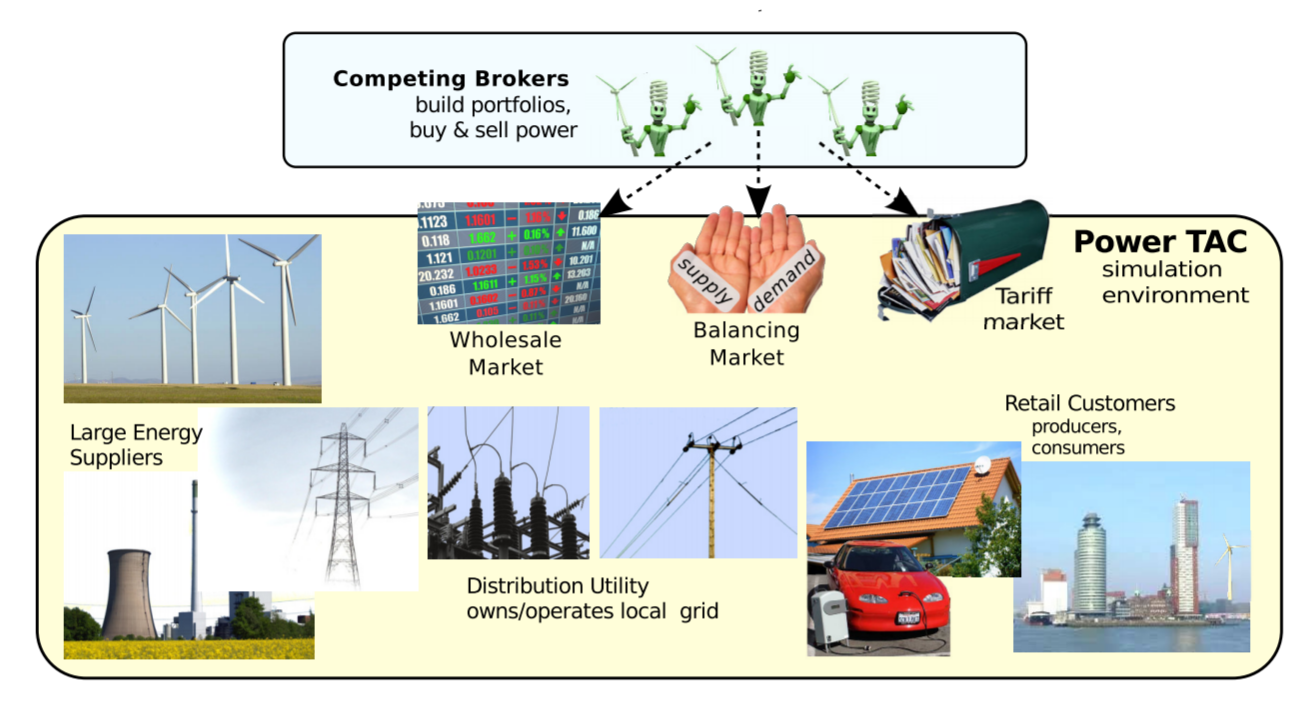
\includegraphics[width=10cm]{img/entorno.png}
    \caption{Elementos del entorno de simulación de Power TAC.}
    \label{entorno}
\end{figure}

A continuación se describen cada uno de los elementos:\\

\textbf{Tiempo de simulación.}\\

El tiempo de simulación en Power TAC se divide por time slot cada uno con una duración de una hora en tiempo de simulación, cada times slot tienen un a duración de 5 segundos en tiempo real, las rondas de simulación consisten en 60 días de simulación equivalente a 1440 timeslot o aproximadamente a 2 horas en tiempo real.\\

\textbf{Customer Market.}\\

También es llamado Mercado de Tarifas, por este medio los agente adquiere energía de los productores locales y la vende a sus consumidores. El agente ofrecen contratos o tarifas especificando el precio y otros términos, mientras que los clientes tomas la decisión de aceptarlos o ignorar. la construcción de una tarifa te permite especificar los siguiente términos: especificar periodo de pagos, tiempo de uso, bonos o pagos por suscripción, mínima duración de contrato, pagos de penalización de retiro antes de cumplir con la mínima duración, precisión por consumo y producción, etc.\\

\textbf{Distribution Utility.}\\

El Distribuidor de Utilidades modela el monopolio regulador que posee y mantiene la infraestructura de distribución de energía. Dentro del contexto de Power TAC, es una tercera entidad responsable de equilibrar la oferta y la demanda en cada intervalo de tiempo a través de un mecanismo de balance.  En Power TAC participa en los siguientes escenarios:

\begin{enumerate}
    \item Encargado de distribuir la energía de la red a los clientes. Implicado pagos por el uso de la distribución de la energía hacia los clientes.
    \item Permite importar y exportar energía desde el Mercado al por Mayor.
    \item 
\end{enumerate}

\textbf{Balancing Market.}\\

El mercado de balance es el encargo de mantener el equilibrio entre la oferta y la demanda en la distribución en la red. el Mercado de Balance mantiene un sistema de incentivo para los broker por mantener el equilibrio entre la oferta y la demanda de su portafolio de clientes en cada intervalo de tiempo. Reduciendo el costo de las penalizaciones de desbalance realizadas por el DU.

\section{Broker.}

El broker es el responsable de ser el intermediario entre las negociaciones en el Mercado de Tarifas, Mercado al por Mayor y el Mercado de Balance, con el objetivo de lograr ganancias a partir de la compra y venta de energía. Durante un times slot el agente puede realizar algunas de las actividades de la figura \ref{activity}.

\begin{figure}[!h]
    \centering
    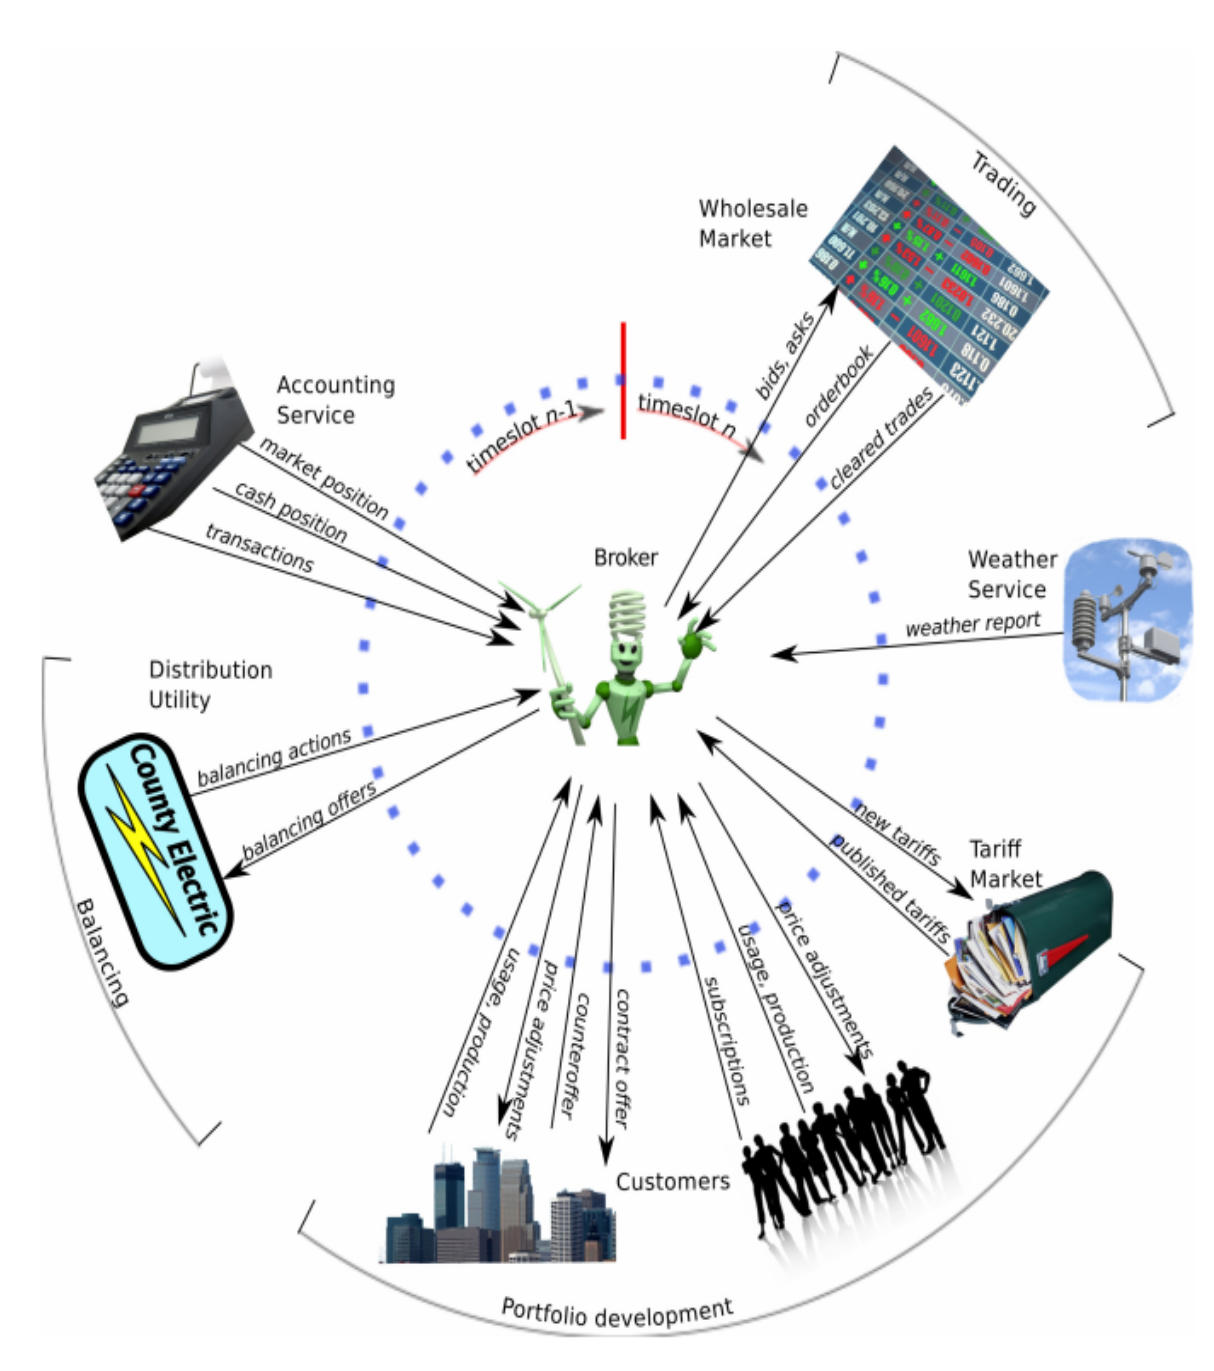
\includegraphics[width=8cm]{img/process.png}
    \caption{Actividades realizadas por el broker en un time slot.}
    \label{activity}
\end{figure}

\begin{description}
    \item [Oferta de tarifas (Mercado de Tarifas):] crea y publica nuevas tarifas.
    \item [Modificación de tarifas (Mercado de Tarifas):]  cambia las condiciones de una tarifa reemplazandola por una nueva.
    \item [Ajuste de precios (Clientes):] ajustar los precios de las tarifas ya existentes.
    \item [Recortar la demanda (Clientes):] para los clientes que han suscrito a las tarifas que permiten capacidades controlables, los broker pueden ejercer restricciones para gestionar la demanda.
    \item [Publicar ordenen de balance (Mercado de Balance):] proporcionar al mercado de balance clientes con capacidades controlables para contribuir al desbalance de la red.
    \item [Enviar solicitudes y ofertas (Mercado al por Mayor):]  crear solicitudes y ofertas para vender y adquirir energía para los futuros time slot.
\end{description}

\section{Tarifas.}
Las tarifas son la relación existente entre un broker y sus clientes, es decir es un contrato que especifica una serie de condiciones asociadas al precio, minima duración de contrato, bonos y pagos por suscripción, penalizaciones por el retiro de un clientes antes de concluir la mínima duración, etc. Los broker son los encargados de crear tarifas específicas a partir de un estructura definida  en la figura \ref{tariff}. La estructura de una tarifa puede variar dependiendo al Power Type que esté sujeta a ella, en la tabla \ref{powertype} muchas las propiedades asociadas a una tarifa dependiendo a que PowerType esta asociado.

\begin{figure}[h!]
    \centering
    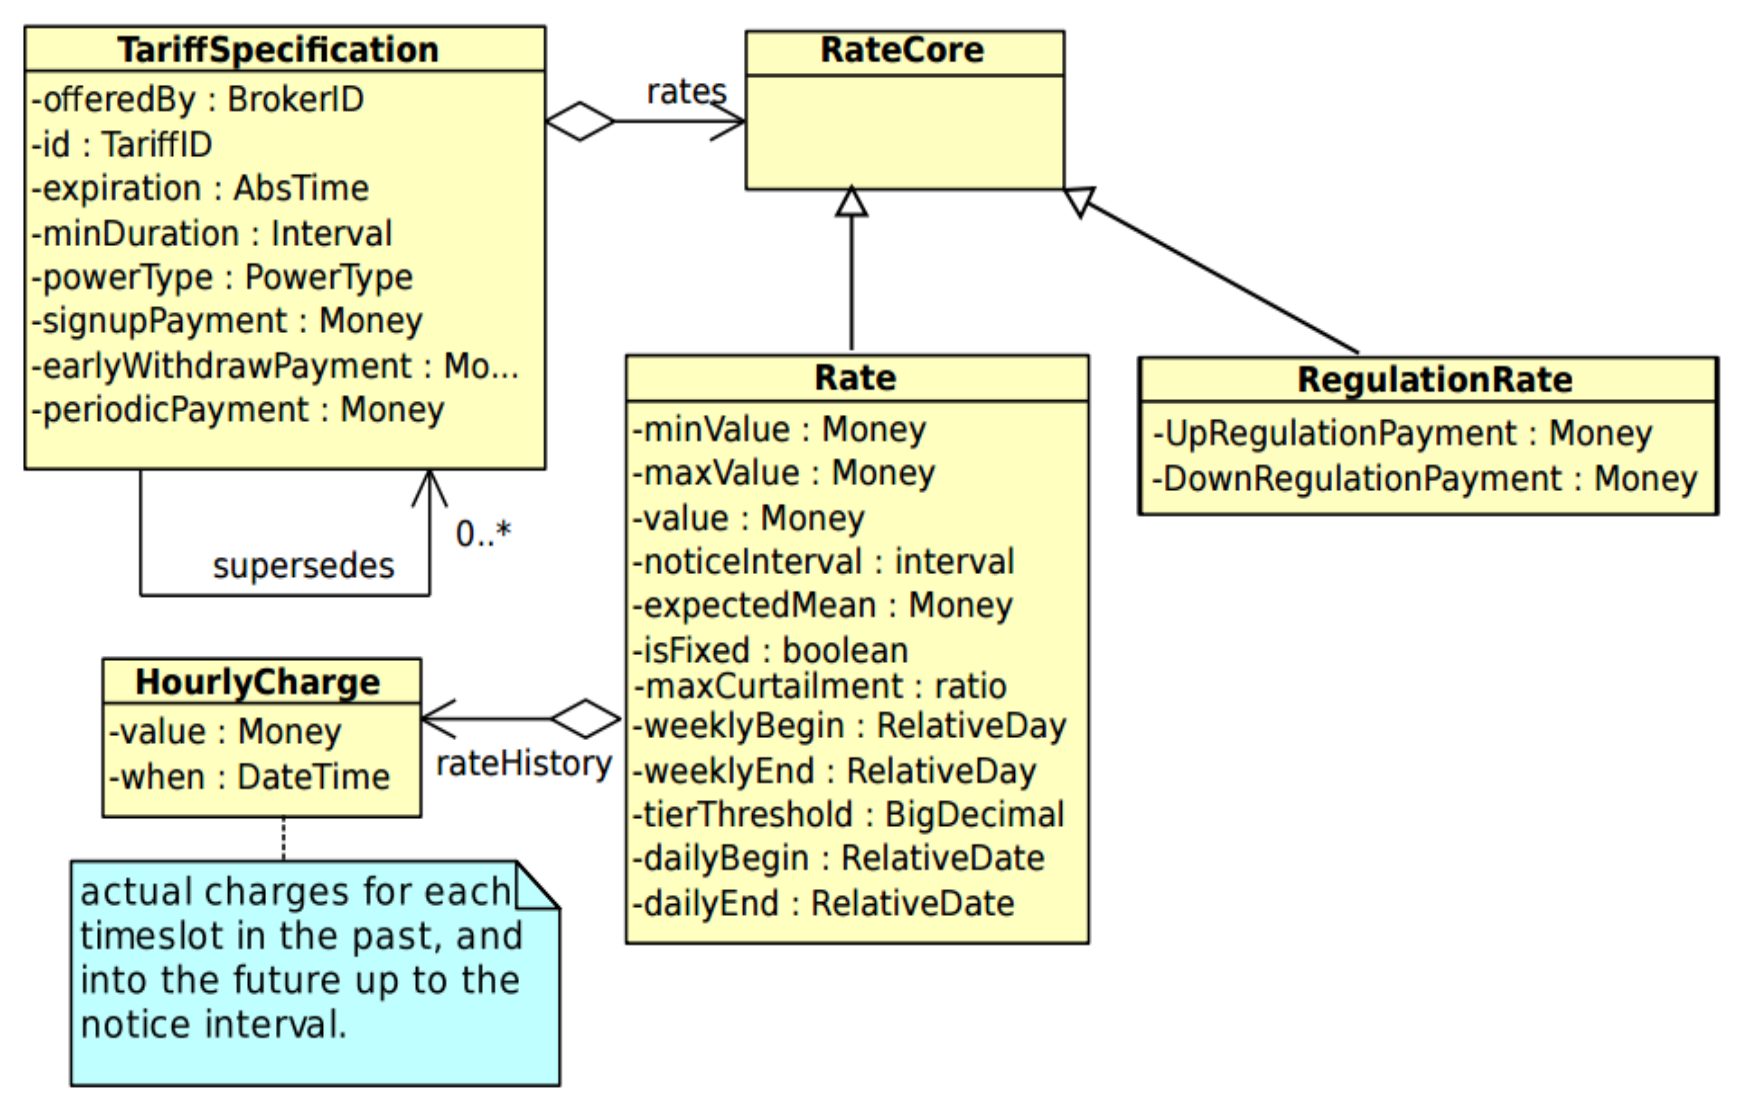
\includegraphics[width=13cm]{img/tariffstructe.png}
    \caption{Clases asociadas a la estructura de una tarifa.}
    \label{tariff}
\end{figure}

